% ACL-style Final Submission Report — self-contained (no acl.sty needed)
% Compile: pdflatex main → pdflatex main

\documentclass[11pt,twocolumn]{article}

% ---- Page geometry (matches ACL template) ----
\usepackage[
  paperwidth=210mm, paperheight=297mm,
  top=25mm, bottom=25mm,
  left=17mm, right=17mm,
  columnsep=6mm
]{geometry}

% ---- Fonts & encoding ----
\usepackage[T1]{fontenc}
\usepackage[utf8]{inputenc}
\usepackage{times}
\usepackage{microtype}

% ---- Math ----
\usepackage{amsmath}
\usepackage{amssymb}

% ---- Tables & figures ----
\usepackage{booktabs}
\usepackage{multirow}
\usepackage{graphicx}
\usepackage{float}
\usepackage{array}
\usepackage{xcolor}

% ---- References ----
\usepackage[round,authoryear]{natbib}

% ---- URLs ----
\usepackage{url}
\usepackage{hyperref}
\hypersetup{colorlinks=true, linkcolor=black, citecolor=black, urlcolor=blue}

% ---- Section style (compact, ACL-like) ----
\usepackage{titlesec}
\titleformat{\section}{\normalfont\large\bfseries}{\thesection}{1em}{}
\titleformat{\subsection}{\normalfont\normalsize\bfseries}{\thesubsection}{1em}{}
\titleformat{\paragraph}[runin]{\normalfont\normalsize\bfseries}{}{0pt}{}[.]
\titlespacing*{\section}{0pt}{8pt}{4pt}
\titlespacing*{\subsection}{0pt}{6pt}{3pt}
\titlespacing*{\paragraph}{0pt}{4pt}{6pt}

% ---- Abstract box ----
\usepackage{abstract}
\setlength{\absleftindent}{0pt}
\setlength{\absrightindent}{0pt}
\renewcommand{\abstractnamefont}{\normalfont\bfseries}

% ---- Caption style ----
\usepackage[font=small,labelfont=bf]{caption}

% ---- Misc layout ----
\setlength{\tabcolsep}{4pt}
\frenchspacing
\setlength{\parindent}{0.25in}
\setlength{\parskip}{0pt}

% --------------------------------------------------------
\title{\Large\bf Multimodal Sentiment and Emotion Analysis via\\[2pt]
Multi-Layer Feature Fusion and Multi-Task Learning\thanks{Code:
\url{https://github.com/Gautam-Gandhi/multimodal-sentiment-analysis}}}

\author{
  \textbf{Manas Inamdar} \\
  2023102052
  \and
  \textbf{Soham Jahagirdar} \\
  2023102046
  \and
  \textbf{Parth Tokekar} \\
  2023102041
  \and
  \textbf{Gautam Gandhi} \\
  2023102059
}

\date{}

\begin{document}
\maketitle

% ============================================================
\begin{abstract}
Multimodal sentiment and emotion analysis aim to infer a speaker's affect by jointly modelling linguistic content, vocal prosody, and facial cues. This report presents a two-phase re-implementation and extension of the UFEN+MTFN architecture of \citet{cai2025multimodal}, a two-stage network that first builds per-modality representations with a Unimodal Feature Extraction Network (UFEN) and then fuses them through six directed cross-modal attention heads and a Transformer encoder--decoder (MTFN). In Phase 1, a fine-tuned BERT text backbone combined with a carefully tuned training recipe reaches MAE = 0.812, Pearson correlation = 0.745, and Acc-2 (np) = 80.3\% on CMU-MOSI after a systematic search over more than 25 configurations. In Phase 2, the same architecture is adapted to 7-way emotion classification on MELD. Nine experiments progressively diagnose and address class collapse, loss scaling, capacity limits, and text dominance. The best result combines a lightweight Multi-Head Feature Tokenization (MHFT) front-end with pre-extracted MultiEMO features, a speaker-disjoint dev split, capped class weights, and a top-5 checkpoint ensemble, yielding weighted F1 = 64.4 and macro F1 = 49.0 with only 3.58M parameters --- surpassing a 111M-parameter BERT-based counterpart on every metric.
\end{abstract}

% ============================================================
\section{Introduction}
\label{sec:intro}

Human communication is inherently multimodal: speakers convey affect through word choice, vocal prosody, and facial expression simultaneously. Multimodal Sentiment Analysis (MSA) and Emotion Recognition in Conversation (ERC) seek to exploit all three channels jointly, rather than relying on text alone. The practical motivation is clear: an utterance such as \emph{``it was fine''} may be semantically neutral, yet a flat vocal delivery and a disappointed facial expression can flip its intended polarity. A unimodal text model has no access to these cues and is therefore limited in ambiguous or sarcastic cases.

Three properties make the problem difficult. First, the three modalities inhabit very different numerical spaces --- contextual word embeddings, prosodic descriptors, and facial action units are not directly comparable. Second, the modalities can carry conflicting signals, a phenomenon central to sarcasm and irony, which requires the model to arbitrate rather than simply average. Third, text is by far the most informative modality for sentiment, which biases learning towards text-only solutions even when the hard cases are precisely those where audio and video would help.

This project re-implements the UFEN+MTFN model of \citet{cai2025multimodal}, which addresses all three issues through a two-stage design. UFEN processes each modality independently using a Bi-GRU, parallel convolutions, and self-attention gating. MTFN then fuses the three representations through six directed cross-modal attention pairs, followed by a Transformer encoder--decoder refinement. Five auxiliary losses (three unimodal and two multimodal) keep every branch informative throughout training.

The project spans two phases. \textbf{Phase 1} (mid-submission) delivers a from-scratch PyTorch implementation on CMU-MOSI, along with a systematic hyperparameter search over more than 25 configurations. \textbf{Phase 2} (this report) adapts the same architecture to 7-class emotion recognition on MELD and reports nine experiments targeting feature scaling, loss design, capacity, text dominance, gradient balancing, and feature representation.

% \paragraph{Contributions.} The principal contributions are as follows:
% \begin{itemize}
%   \item A reproducible PyTorch implementation of UFEN+MTFN in which every architectural choice is documented, including decisions where the original paper is ambiguous.
%   \item A tuned CMU-MOSI configuration reaching MAE = 0.812, Corr = 0.745, and Acc-2 (np) = 80.3\%, alongside a component ablation confirming the contribution of cross-modal attention, multi-task unimodal losses, and the encoder--decoder.
%   \item A complete Phase 2 experiment trail on MELD (Exp 1--9.1): feature normalization, loss design, video projection, capacity sweeps, BERT fine-tuning, bimodal/unimodal ablations, a stacked OGM-GE + InfoNCE + scheduled-unfreeze run, and finally a Multi-Head Feature Tokenization (MHFT) front-end that adapts UFEN to pre-pooled MultiEMO features.
%   \item A best MELD result of weighted F1 = 64.4 and macro F1 = 49.0, obtained by the MHFT variant with 3.58M parameters --- roughly 30$\times$ smaller and 4$\times$ faster to train than the BERT-based Exp 6.
%   \item A transparent account of three changes that did not work (focal loss, doubled capacity, curriculum-style unfreezing) and the dataset-level reasons they failed.
% \end{itemize}

% ============================================================
\section{Related Work}
\label{sec:related}

\paragraph{Unimodal representations} Early MSA systems relied on hand-crafted features such as n-gram frequencies, pitch statistics, and facial action units. Recurrent models (LSTM, GRU) subsequently provided learned sequence representations \citep{poria2017review}, and pre-trained contextual encoders, most notably BERT \citep{devlin2019bert}, substantially improved text quality by assigning context-dependent embeddings --- a property that matters for polarity-shifting phrases such as \emph{``that performance was sick''}. For CMU-MOSI and MELD, COVAREP \citep{degottex2014covarep}, Wave2Vec2.0, FACET, and ResNet features are the standard upstream extractors.

\paragraph{Fusion strategies.} Early fusion concatenates modality vectors before learning. Tensor Fusion \citep{zadeh2017tensor} instead forms the outer product of modality vectors, capturing pairwise and triple interactions explicitly at a cost that grows as $d^3$; LMF \citep{liu2018efficient} factorises this tensor to control computation. Late fusion trains independent per-modality classifiers and combines their decisions. Attention-based fusion is now dominant: MulT \citep{tsai2019multimodal} applies cross-modal attention so that each modality attends to every time step of the others; MFN \citep{zadeh2018memory} stores multi-view interactions in an explicit memory; and MISA \citep{hazarika2021misa} decomposes each modality into shared and modality-specific subspaces.

\paragraph{Multi-task learning for sentiment.} Because text tends to dominate the learning signal, models often rely on the language branch and neglect audio and video. Multi-task learning counteracts this: Self-MM \citep{yu2021selfmm} constructs unimodal labels through a self-supervised procedure and supervises a head per modality, while MMIM \citep{han2021improving} maximises mutual information between modality features and the final prediction. UFEN+MTFN \citep{cai2025multimodal} combines cross-modal attention in the spirit of MulT with multi-task learning in the spirit of Self-MM, and additionally refines the fused representation via a Transformer encoder--decoder.

\paragraph{Emotion recognition in conversation.} MELD \citep{poria2019meld} contains dialogue clips from the sitcom \emph{Friends}, annotated with seven emotion categories. Subsequent work such as DialogueRNN, DialogueGCN, and MM-DFN models inter-utterance context within a dialogue. Much of this literature relies on strong pre-extracted features rather than raw modalities, and the MultiEMO release \citep{shi2023multiemo} provides a standard feature set comprising RoBERTa (text), openSMILE-derived (audio), and DenseNet (video) utterance-level representations.

% ============================================================
\section{Datasets}
\label{sec:dataset}

\subsection{CMU-MOSI (Phase 1)}

CMU-MOSI \citep{zadeh2016multimodal} contains 2{,}199 short utterances extracted from YouTube movie reviews, each annotated with a continuous sentiment score in $[-3, +3]$. The splits are fixed at 1{,}283 / 214 / 686 for train, validation, and test respectively. Phase 1 uses a fine-tuned \texttt{bert-base-uncased} encoder (768-dim contextual embeddings) for text, 74-dimensional COVAREP features for audio, and 47-dimensional FACET features for visual, each padded per utterance.

The COVAREP features contain placeholder values near $-3.4 \times 10^{38}$ in silent frames. Preprocessing clips values to $[-10^4, 10^4]$, replaces remaining non-finite entries with zero, and applies $Z$-score normalisation using training-set statistics only.

\subsection{MELD (Phase 2)}

MELD \citep{poria2019meld} contains 13{,}708 utterances from \emph{Friends}, labelled with seven emotions: Neutral, Surprise, Fear, Sadness, Joy, Disgust, and Anger. The label distribution is strongly skewed: Neutral accounts for approximately 47\% of training samples, while Fear and Disgust each contribute under 3\%. The standard splits are 9{,}988 / 1{,}108 / 2{,}610.

Phase 2 uses two feature sets on MELD:
\begin{itemize}
  \item \textbf{MM-Align features (Exp 1--8):} GloVe 300-dim text (Exp 1--5), Wave2Vec2.0 32-dim audio, and ResNet-101 2048-dim video, all provided as time-aligned sequences.
  \item \textbf{MultiEMO features (Exp 9, 9.1):} RoBERTa-base 768-dim text, openSMILE-derived 512-dim audio, and DenseNet 1000-dim video, each released as a single utterance-level vector.
\end{itemize}

% ============================================================
\section{Methodology}
\label{sec:method}

\subsection{Task Definitions}

\textbf{Phase 1 (CMU-MOSI)} is a regression task: given the three modality sequences, the model predicts a scalar sentiment score in $[-3, +3]$. All five heads ($Y_t$, $Y_a$, $Y_v$, $Y_m$, $Y_{m'}$) are trained with mean squared error, and $Y_{m'}$ is used as the final prediction at test time.

\textbf{Phase 2 (MELD)} is a 7-way classification task: the same five heads output class logits, and the loss is a weighted sum of cross-entropy terms with label smoothing and inverse-frequency class weights.

\subsection{Architecture Overview}

The overall pipeline is identical across both phases and proceeds in two stages (Fig.~\ref{fig:arch}). Stage 1 (UFEN) builds a representation for each modality independently. Stage 2 (MTFN) fuses the three representations through cross-modal attention and a Transformer encoder--decoder. Only the output head differs between phases: linear regression for CMU-MOSI and a softmax classifier for MELD. Phase 2 additionally introduces an optional MHFT front-end that allows UFEN to ingest utterance-level features.

\begin{figure}[t]
\centering
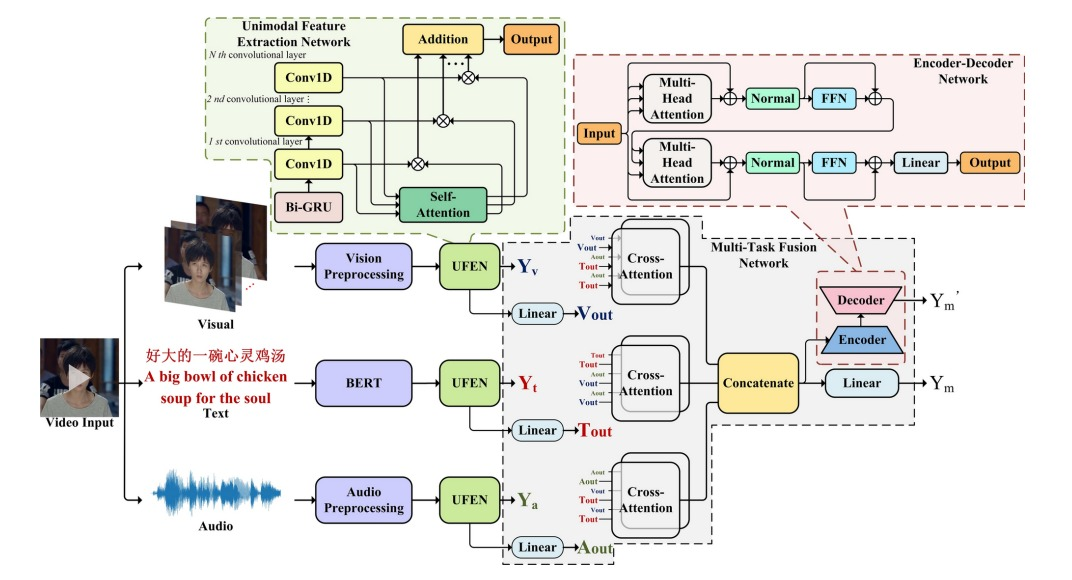
\includegraphics[width=1.0\linewidth]{figures/arch.png}
\caption{The UFEN+MTFN architecture. Each UFEN independently encodes one modality via Bi-GRU, parallel convolutions, and self-attention gating, producing a unimodal prediction ($Y_t, Y_a, Y_v$). MTFN fuses the three representations via six directed cross-modal attention pairs, then refines the result through a Transformer encoder--decoder to obtain the final output $Y_{m'}$.}
\label{fig:arch}
\end{figure}

\subsection{Stage 1: UFEN}
\label{sec:ufen}

UFEN proceeds through five stages. Each modality has its own instance with independent parameters.

\paragraph{1. Bi-GRU.}
\begin{equation}
X_i^{\text{BiGRU}} = \text{BiGRU}(X_i) \in \mathbb{R}^{T \times d_m}
\end{equation}
A bidirectional recurrent pass captures context from both directions, which is important for constructions such as \emph{``not bad at all''} whose polarity depends on subsequent tokens.

\paragraph{2. Parallel Conv1Ds.}
\begin{equation}
X_i^{\ell} = \text{Conv1D}^{\ell}\!\left(X_i^{\text{BiGRU}},\; K_\ell,\; F\right)
\end{equation}
for $\ell = 1, \ldots, l$ parallel branches. Each branch captures temporal patterns at a distinct scale. Phase 1 uses $l=2$ with kernels $[1, 5]$, so one branch preserves per-token information while the other captures 5-step context; Phase 2 adopts the same configuration.

\paragraph{3. Self-attention gating.}
\begin{align}
\text{Att}(X) &= \text{softmax}\!\left(\tfrac{X X^\top}{\sqrt{d_k}}\right) X \\
X_i^{\text{self-att},\ell} &= X_i^{\ell} \otimes \text{Att}(X_i^{\ell})
\end{align}
where $\otimes$ denotes element-wise multiplication. The attention output is used as a multiplicative gate rather than an additive residual, amplifying salient time steps within each branch.

\paragraph{4. Unpool and sum.}
\begin{equation}
X_i^{\text{fusion}} = \sum_{\ell=1}^{l} W_\ell \, X_i^{\text{self-att},\ell}
\end{equation}
Summing across branches preserves multi-scale information in the fused representation.

\paragraph{5. Unimodal head.}
\begin{equation}
Y_i = W_i \cdot \text{MeanPool}(X_i^{\text{fusion}}) + b_i
\end{equation}
This prediction is used only during training, as part of the multi-task loss, and obliges each UFEN branch to be individually predictive.

\subsection{Stage 2: MTFN}
\label{sec:mtfn}

\paragraph{Cross-modal attention.} For every ordered pair $(i, j)$ of modalities, both sequences are projected to a shared dimension and processed by multi-head attention using modality $i$ as query and modality $j$ as key/value:
\begin{equation}
\text{CA}_{i \to j} = \text{LN}\!\left(\text{MHAtt}(Q_i, K_j, V_j)\right)
\end{equation}
All six directed pairs are computed.

\paragraph{First multimodal prediction.} Each attention output is mean-pooled over the query modality's time dimension and concatenated:
\begin{equation}
\text{Fused} = \text{Concat}\!\left[\text{MeanPool}(\text{CA}_{i \to j})\right] \in \mathbb{R}^{6 d_m},
\end{equation}
and a linear projection produces the first multimodal prediction $Y_m$.

\paragraph{Transformer encoder--decoder.} The fused vector is reshaped into a length-6 sequence and refined through one encoder block and one decoder block:
\begin{align}
\text{Out}_{\text{enc}} &= \text{Encoder}(\text{Fused}), \\
\text{Out}_{\text{dec}} &= \text{Decoder}(\text{Fused}, \text{Out}_{\text{enc}}).
\end{align}
Mean pooling followed by a linear layer yields the final prediction $Y_{m'}$, which is used at test time.

\subsection{Multi-Task Loss}

All five heads are trained jointly. Phase 1 uses MSE, while Phase 2 uses weighted cross-entropy with label smoothing:
\begin{equation}
\mathcal{L}_{\text{total}} = \mathcal{L}_t + \mathcal{L}_a + \mathcal{L}_v + \mathcal{L}_m + \mathcal{L}_{m'}.
\end{equation}
The three unimodal losses are essential: without them, the model quickly relies almost exclusively on text, since text alone already yields a competitive error.

\subsection{Phase 2 Extensions}

\paragraph{BERT text encoder (Exp 6 onwards).} The GloVe embedding is replaced with \texttt{bert-base-uncased}, fine-tuned end-to-end with \texttt{lr\_bert} = $2 \times 10^{-5}$, a 3-epoch linear warmup, and cosine decay; the remainder of the model uses \texttt{lr} = $10^{-3}$. Mixed-precision training and a reduced batch size are required to fit BERT on a single RTX 3050.

\paragraph{OGM-GE + InfoNCE + scheduled training (Exp 8).} Three research-motivated components are added on top of Exp 6 to mitigate text dominance:
(i) \textbf{OGM-GE} \citep{peng2022ogmge}, which measures the gradient norm on each UFEN branch after the backward pass and rescales weaker branches towards the strongest, capped at $10\times$;
(ii) \textbf{symmetric cross-modal InfoNCE} \citep{vandenoord2018cpc} applied to pooled UFEN embeddings of every modality pair, with temperature 0.07 and weight $\lambda_{\text{align}} = 0.1$;
(iii) a three-phase schedule that first pre-trains audio and video alone (with text and MTFN frozen), then unfreezes all unimodal heads while keeping MTFN frozen, and finally releases the full model with the five-task loss.

\paragraph{Multi-Head Feature Tokenization (Exp 9, 9.1).} MultiEMO features are released at the utterance level --- a single vector per clip --- which is incompatible with UFEN's sequence-oriented pipeline. Rather than modifying UFEN, a small front-end is added:
\begin{equation}
\text{MHFT}(x) = \text{reshape}(W x + b) + P \;\in\; \mathbb{R}^{K \times d_m},
\end{equation}
where $x$ is the utterance vector, $W$ produces $K \cdot d_m$ outputs, $P$ is a learned positional embedding, and the result is a synthetic length-$K$ token sequence with $K = 8$. UFEN and MTFN operate on this sequence without any modification. MHFT is the sole new component: the UFEN and MTFN modules are byte-for-byte identical to Phase 1.

\paragraph{Speaker-disjoint dev split, capped class weights, and ensemble (Exp 9.1).} The public MultiEMO pickle does not provide a dev split, so Exp 9 randomly partitioned \texttt{trainVid} 90/10. This left the six main \emph{Friends} characters represented in both train and dev, allowing the model to memorise speaker-specific patterns and producing an inflated dev F1w (71.7) that did not transfer to test (61.5). Exp 9.1 therefore (i) holds out entire dialogue groups keyed by their dominant speaker, starting from rarer speakers; (ii) caps inverse-frequency class weights at 1.5, affecting only Fear and Disgust (previously 2.24 and 2.41); and (iii) averages softmax probabilities over the top-5 dev checkpoints at test time.

% ============================================================
\section{Experimental Setup}
\label{sec:setup}

\paragraph{Implementation.} All models are implemented in PyTorch 2.0. Phase 1 runs on an RTX 3050 Laptop GPU with approximately three minutes per training run. Phase 2 BERT experiments run on a Kaggle T4. The code is organised into per-component modules, and JSON configuration files control hyperparameters so that experiments can be swept without code changes.

\paragraph{Metrics (CMU-MOSI).} Following \citet{yu2021selfmm}, six metrics are reported: Acc-2 nn/np (binary accuracy computed on all samples / non-zero samples), F1 nn/np, mean absolute error (MAE; lower is better), Pearson correlation, and Acc-7 (integer-rounded 7-way accuracy).

\paragraph{Metrics (MELD).} Following the standard MELD protocol, weighted F1 (\textbf{F1w}, the headline metric), macro F1 (\textbf{F1m}, sensitive to rare classes), and accuracy are reported, together with per-class F1 and confusion matrices.

\paragraph{Phase 2 baseline hyperparameters.} Unless otherwise specified: $d_m = 128$, convolution dimensions $[64, 64]$ with kernels $[1, 5]$, $d_{\text{ff}} = 128$, one self-attention head, four cross-attention heads, attention dropout 0.2, dropout 0.1, batch size 32, Adam optimiser, cosine learning-rate schedule with early-stopping patience 10, gradient clipping at norm 1.0, inverse-frequency class weights, and label smoothing 0.1.

% ============================================================
\section{Results}
\label{sec:results}

\subsection{Phase 1: CMU-MOSI}

Phase 1 involved more than 25 configurations organised into three sub-phases. Phase~1a varied individual hyperparameters (learning rate for BERT, $d_m$, $d_{\text{ff}}$, convolution kernels, gradient clipping) from a paper-matching baseline. Phase~1b combined the winners and identified cosine LR scheduling with early stopping at patience 15 as the single largest improvement. Phase~1c targeted the remaining dev/test gap with regularisation: weight decay was catastrophic for BERT fine-tuning on a small dataset, whereas a 5-epoch linear warmup for the BERT learning rate eliminated early-training instability and produced the cleanest convergence curve. The resulting configuration, referred to as P3-2, uses $d_m = 128$, $d_{\text{ff}} = 128$, kernels $[1, 5]$, \texttt{lr} = $5 \times 10^{-3}$ for non-BERT parameters, \texttt{lr\_bert} = $2 \times 10^{-5}$, cosine annealing for both learning rates, and BERT warmup over 5 epochs.

\begin{table}[h]
\centering
\small
\begin{tabular}{lcc}
\toprule
\textbf{Metric} & \textbf{Ours (P3-2)} & \textbf{Paper} \\
\midrule
MAE $\downarrow$           & \textbf{0.812} & 0.728 \\
Pearson Correlation $\uparrow$ & \textbf{0.745} & 0.792 \\
Acc-7 $\uparrow$           & \textbf{43.0}  & 46.7 \\
Acc-2 nn $\uparrow$        & \textbf{78.6}  & 85.2 \\
Acc-2 np $\uparrow$        & \textbf{80.3}  & 86.6 \\
F1 np $\uparrow$           & \textbf{80.4}  & 86.7 \\
\bottomrule
\end{tabular}
\caption{CMU-MOSI test results for the best Phase 1 configuration compared against the paper's reported numbers. The model has approximately 110.8M trainable parameters (dominated by BERT).}
\label{tab:mosi_results}
\end{table}

The P3-2 configuration reaches MAE = 0.812, Pearson correlation = 0.745, and Acc-2 (np) = 80.3\% on the CMU-MOSI test set (Table~\ref{tab:mosi_results}). The dev-set MAE reached 0.7434 at epoch 42, within 0.015 of the paper's reported test MAE of 0.728, indicating that the remaining gap is primarily a dev-to-test generalisation issue rather than a capacity or training limitation on a dataset of 1{,}283 training samples.

\paragraph{Phase 1 component ablation.} Table~\ref{tab:mosi_ablation} reports an ablation over the key architectural components. Each component contributes a measurable improvement.

\begin{table}[h]
\centering
\small
\begin{tabular}{lcc}
\toprule
\textbf{Configuration} & \textbf{Acc-2 (np)} & \textbf{Corr} \\
\midrule
Full model (P3-2)                   & \textbf{80.3} & \textbf{0.745} \\
No cross-modal attention            & 76.0          & 0.688 \\
No unimodal losses                  & 77.8          & 0.714 \\
No encoder--decoder                  & 78.7          & 0.728 \\
Single UFEN convolution branch      & 75.7          & 0.708 \\
\bottomrule
\end{tabular}
\caption{Phase 1 ablation on CMU-MOSI. Cross-modal attention contributes the largest single improvement.}
\label{tab:mosi_ablation}
\end{table}

Removing cross-modal attention, and replacing it with simple concatenation of mean-pooled UFEN outputs, produces the largest drop (Acc-2 np: $-4.3$ points). Dropping the three unimodal losses reduces Acc-2 (np) by 2.5 points, confirming that multi-task supervision prevents the model from collapsing onto the text signal. The encoder--decoder adds a further 1.6 points on top. The convolution branch sweep replicates the paper's finding that two parallel branches outperform a single branch.

\subsection{Phase 2: MELD --- Experiment Trail}

Table~\ref{tab:meld_summary} summarises the nine Phase 2 experiments; Table~\ref{tab:meld_perclass} provides per-class F1 values. Each experiment is discussed below.

\begin{table*}[t]
\centering
\small
\begin{tabular}{lcccccc}
\toprule
\textbf{Exp} & \textbf{Description} & \textbf{Acc} & \textbf{F1w} & \textbf{F1m} & \textbf{Params} & \textbf{Best ep} \\
\midrule
1    & Baseline (direct port of Phase 1 hparams)  & 47.7 & 42.0 & 19.6 & 3.84M & 8 \\
2    & + LayerNorm + lr $10^{-3}$ + smoothing     & 50.4 & 51.4 & 33.1 & 3.85M & 9 \\
3    & + Video proj + Focal loss + lr $5\!\!\times\!\!10^{-4}$ + dropout 0.2 & 51.4 & 50.5 & 31.7 & 3.68M & 46 \\
4    & Exp 3 with CE instead of Focal             & 49.8 & 50.3 & 31.9 & 3.68M & 20 \\
5    & Exp 2 with $d_m = 256$                     & 51.0 & 50.3 & 29.7 & 7.12M & 3 \\
6    & Exp 2 + BERT text encoder                  & \textbf{61.0} & 60.3 & 42.8 & 111.4M & 7 \\
7a   & Exp 6, text + audio only                   & 56.3 & 59.1 & 43.8 & 110.4M & 3 \\
7b   & Exp 6, text + video only                   & 57.7 & 59.5 & 43.8 & 111.0M & 4 \\
7c   & Exp 6, text only                           & 55.9 & 57.9 & 42.7 & 109.5M & 4 \\
8    & Exp 6 + OGM-GE + InfoNCE + scheduled       & 60.3 & 59.4 & 43.3 & 111.4M & 18 \\
9    & MHFT + MultiEMO (random dev split)         & 60.0 & 61.5 & 45.7 & 3.58M & 10 \\
\textbf{9.1} & \textbf{Exp 9 + speaker split + capped wts + top-5 ensemble} & 63.2 & \textbf{64.4} & \textbf{49.0} & \textbf{3.58M} & 6 \\
\bottomrule
\end{tabular}
\caption{MELD test results across all Phase 2 experiments. F1w is the primary metric. Exp 9.1 is the best overall configuration.}
\label{tab:meld_summary}
\end{table*}

\begin{table*}[t]
\centering
\small
\begin{tabular}{lccccccc}
\toprule
\textbf{Exp} & Neutral & Surprise & Fear & Sadness & Joy & Disgust & Anger \\
\midrule
1    & 0.71 & 0.31 & 0.00 & 0.00 & 0.00 & 0.00 & 0.35 \\
2    & 0.68 & 0.49 & 0.08 & 0.22 & 0.47 & 0.06 & 0.32 \\
3    & 0.69 & 0.46 & 0.10 & 0.19 & 0.44 & 0.07 & 0.27 \\
4    & 0.67 & 0.48 & 0.05 & 0.20 & 0.45 & 0.07 & 0.31 \\
5    & 0.71 & 0.47 & 0.00 & 0.23 & 0.46 & 0.07 & 0.14 \\
6    & 0.76 & 0.53 & 0.17 & 0.27 & 0.58 & 0.23 & 0.46 \\
7a   & 0.70 & 0.57 & 0.10 & 0.37 & 0.62 & 0.25 & 0.46 \\
7b   & 0.73 & 0.55 & 0.16 & 0.31 & 0.57 & 0.28 & 0.47 \\
7c   & 0.70 & 0.56 & 0.16 & 0.30 & 0.57 & 0.24 & 0.45 \\
8    & 0.75 & 0.52 & 0.19 & 0.29 & 0.58 & 0.29 & 0.41 \\
9    & 0.74 & 0.57 & 0.19 & 0.35 & 0.63 & 0.25 & 0.47 \\
\textbf{9.1} & \textbf{0.77} & 0.56 & \textbf{0.20} & \textbf{0.43} & 0.62 & \textbf{0.32} & \textbf{0.51} \\
\bottomrule
\end{tabular}
\caption{Per-class F1 scores on the MELD test set. Exp 9.1 achieves the best or tied-best score on five of seven classes.}
\label{tab:meld_perclass}
\end{table*}

\paragraph{Exp 1 --- Baseline.} A direct port of the Phase 1 hyperparameters with the regression head replaced by a classifier produced a degenerate model: predictions collapsed onto Neutral and Anger, and the remaining five classes received F1 = 0. Three factors were identified. First, the Phase 1 learning rate of $5 \times 10^{-3}$ was too high for MELD, causing dev F1w to oscillate violently (35 $\to$ 6 $\to$ 35 $\to$ 25 $\to$ 36). Second, GloVe text features had an $L_2$ norm near 5, compared with 0.85 for audio and 0.72 for video, yielding a roughly sevenfold text dominance in the raw input. Third, the optimiser converged to a trivial local minimum in which predicting the two majority classes was locally optimal.

\paragraph{Exp 2 --- The fix.} Three modifications were introduced: a per-modality LayerNorm applied before UFEN to equalise feature scales; a reduced learning rate of $10^{-3}$; and label smoothing 0.1 to discourage overconfident majority-class predictions. The class collapse was resolved, all seven classes received predictions, and F1w improved by $+9.4$ points (42.0 $\to$ 51.4) while F1m improved by $+13.5$ points (19.6 $\to$ 33.1). Exp 2 became the GloVe baseline.

\paragraph{Exp 3--5 --- Attempts that did not help.} Three subsequent modifications reduced weighted F1. \textbf{Exp 3} introduced a linear projection from 2048 to 256 dimensions before the video BiGRU, a focal loss with $\gamma = 2$, and a lower learning rate; the focal penalty was too aggressive, sacrificing mid-frequency classes (Anger, Sadness) for marginal gains on Fear and Disgust. \textbf{Exp 4} retained the video projection but reverted to cross-entropy; the combination of explicit projection and lower learning rate still underperformed Exp 2's direct BiGRU-on-2048 pipeline. \textbf{Exp 5} doubled $d_m$ to 256 and $d_{\text{ff}}$ to 256; training became unstable (dev F1w oscillated between 35 and 46), the best epoch was 3, and Anger collapsed to F1 = 0.14. These results indicated that the plateau at approximately 51 F1w was a feature-quality limitation rather than an architectural one: context-free GloVe embeddings cannot disambiguate sarcastic from agreeable uses of the same tokens.

\paragraph{Exp 6 --- BERT breaks the ceiling.} Replacing GloVe with a fine-tuned \texttt{bert-base-uncased} improved F1w from 51.4 to \textbf{60.3} ($+8.9$) and F1m from 33.1 to \textbf{42.8} ($+9.7$). Every class improved, with the largest gains on mid-frequency classes where text ambiguity is most detrimental: Joy ($+0.11$), Disgust ($+0.16$), and Anger ($+0.14$). Fear produced non-zero F1 for the first time (0.17). The cost was a 111M-parameter model with approximately 45 seconds per epoch.

\paragraph{Exp 7 --- Bimodal and unimodal ablations.} The contribution of each modality was quantified by rerunning Exp 6 with pairs and singletons. \textbf{Text-only (7c)} already reached F1w = 57.9, indicating that audio and video together contribute only $+2.4$ F1w on top of BERT. Text+audio (7a) and text+video (7b) each added approximately $+1.2$ over text alone and were roughly tied. Audio was more informative for Sadness (F1 = 0.37 vs.\ 0.27 in the full 3-modal system), where prosodic cues such as low pitch and reduced energy are characteristic, while video was more informative for Neutral, where facial grounding helps distinguish neutrality from Sadness and Fear. The limited gain from audio and video reflects the nature of MELD: \emph{Friends} is scripted dialogue in which writers encode emotion primarily through word choice.

\paragraph{Exp 8 --- OGM-GE + InfoNCE + scheduled unfreezing.} In principle, this combination --- balanced multimodal learning via gradient modulation \citep{peng2022ogmge}, cross-modal contrastive alignment \citep{vandenoord2018cpc}, and a curriculum over modality unfreezing --- should help the weaker branches. In practice the result was essentially neutral: F1w 60.3 $\to$ 59.4 ($-0.9$) and F1m 42.8 $\to$ 43.3 ($+0.5$). The curriculum was particularly revealing. During Phase A (epochs 1--3), with text and MTFN frozen, audio and video alone made no measurable progress: accuracy remained near 2\% and F1w near 0.1\%. The Wave2Vec2-32 and ResNet-101 features simply do not carry first-order class information in isolation on MELD; their contribution is unlocked only when conditioned on text. Phase B (unfrozen text, frozen MTFN) reached only F1w = 10.5, and Phase C recovered the Exp 6 level by epoch 18 --- eleven epochs later than the baseline. The small gains on Disgust ($+0.06$), Fear ($+0.02$), and Sadness ($+0.02$) cannot be cleanly attributed to any single mechanism, as all three interventions were stacked. The broader lesson is that curricula assuming weaker modalities can bootstrap alone fail when those modalities do not carry isolated class signal.

\paragraph{Exp 9 --- MHFT with MultiEMO features.} Substituting utterance-level MultiEMO \citep{shi2023multiemo} features (RoBERTa-768, openSMILE-512, DenseNet-1000) via the MHFT front-end proved to be the most impactful change of the project. The UFEN and MTFN modules remained unchanged; MHFT added 2.3M parameters. Because the BERT backbone was removed entirely, the total parameter count dropped from 111M to \textbf{3.58M}. Despite this 30$\times$ reduction, F1w improved to 61.5 (best so far) and F1m to 45.7 (also best so far). Every minority class improved: Sadness $+0.08$, Joy $+0.05$, Surprise $+0.04$, Fear $+0.02$, Disgust $+0.02$. Training was also approximately four times faster, at roughly 10 seconds per epoch. However, dev F1w reached 71.7 while test reached only 61.5 --- a 10-point generalisation gap.

\paragraph{Exp 9.1 --- Closing the gap.} Investigation revealed that the random 90/10 split of \texttt{trainVid} was leaking speaker and scene context. Because \emph{Friends} is dominated by six main characters, a random dialogue split leaves all characters represented in both train and dev, allowing the model to memorise speaker-specific phrasing and prosody. Three changes were introduced: (i) a \textbf{speaker-disjoint dev split} holding out entire dialogue groups keyed by their dominant speaker; (ii) \textbf{capped class weights} at 1.5, affecting only Fear and Disgust (previously 2.24 and 2.41); and (iii) a \textbf{top-5 checkpoint ensemble} averaging softmax probabilities over the five best dev epochs. Together, these changes closed the dev-to-test gap from 10.2 to 5.7 points and improved test F1w to \textbf{64.4} and F1m to \textbf{49.0} --- the best result overall. Notably, the training set shrank from 9{,}920 to 6{,}464 samples, so the gain reflects improved generalisation rather than additional data. Each fix is individually identifiable: the speaker-disjoint split aligned dev and test signals (dev F1w dropped 71.7 $\to$ 70.1 while test rose 61.5 $\to$ 64.3); the capped weights reduced Neutral-to-Fear false positives from 84 to 43 (a 49\% decrease); and the ensemble added $+0.1$ F1w and $+0.9$ F1m over the single-best checkpoint.

% ============================================================
\section{Analysis}
\label{sec:analysis}

\subsection{Positive Results}

\paragraph{Every component of UFEN+MTFN is justified.} Phase 1 ablations demonstrate that cross-modal attention, multi-task unimodal losses, and the Transformer encoder--decoder each contribute measurably. Cross-modal attention is the most consequential: its removal alone reduces Acc-2 by 4.3 points on MOSI.

\paragraph{BERT is the dominant lever on MELD.} Replacing GloVe with fine-tuned BERT produced an $+8.9$-point improvement in weighted F1 in a single change. Context-free embeddings are the principal bottleneck for emotion classification on scripted dialogue.

\paragraph{MHFT offers a favourable trade-off.} Utterance-level MultiEMO features processed by an 8-token MHFT front-end outperform the full BERT model on every metric (F1w 64.4 vs.\ 60.3; F1m 49.0 vs.\ 42.8), with 30$\times$ fewer parameters and 4$\times$ faster training. The core UFEN+MTFN stack is reused without modification. This pattern is attractive in practice: pre-extracted features can be computed once, and a compact MHFT+UFEN+MTFN model can then be trained in minutes per epoch.

\paragraph{Evaluation integrity is consequential.} Exp 9 and Exp 9.1 share the same architecture and hyperparameters. The only differences are how the dev set is constructed and how checkpoints are selected and combined. These changes alone moved F1w by 2.9 points and F1m by 3.3 points. A naive split would have understated the true quality of the method.

\subsection{Negative Results}

\paragraph{Focal loss is counter-productive here.} With $\gamma = 2$, focal loss over-penalises easy Neutral and Joy examples, degrading mid-frequency classes for marginal gains on Fear and Disgust. Weighted cross-entropy with label smoothing consistently produced better weighted F1.

\paragraph{Doubling capacity destabilises small-dataset training.} A model with $d_m = 256$ (7.1M parameters) on 10K MELD samples was severely unstable, and its best epoch was the third. The effective capacity sweet spot is approximately 3.8M parameters for the GloVe baseline and under 4M for MHFT. BERT's 111M parameters are tolerable only because most are pre-trained.

\paragraph{Curriculum unfreezing fails when weak modalities cannot bootstrap.} Phase A of Exp 8, which trained audio and video with text frozen, produced no measurable learning over three epochs. This offers a concrete counter-example to the assumption behind gradient-blending-style curricula: when a modality carries no first-order class signal in isolation, giving it a head start alone does not recover it.

\paragraph{Explicit video projection discards information.} Projecting ResNet-101 2048-dim features to 256 dimensions before UFEN reduced F1w. The BiGRU's implicit 2048 $\to$ 64 compression appears to perform end-to-end channel selection, which a fixed linear projection cannot replicate.

\subsection{Error Analysis}

The confusion matrix of Exp 9.1 reveals three persistent error patterns.

\paragraph{Neutral absorbs minority-class errors.} Approximately 7--10\% of every non-Neutral class is misclassified as Neutral (for example, 40 Sadness, 59 Joy, and 44 Anger utterances). This follows naturally from Neutral comprising 48\% of the test set combined with the inherent ambiguity of short utterances.

\paragraph{Anger, Surprise, and Joy form a fuzzy triangle.} The three high-arousal classes overlap considerably in prosody (raised pitch, higher energy), and Anger-Surprise confusion is bidirectional.

\paragraph{Fear and Disgust remain difficult.} With only 50 and 68 test samples respectively, per-class F1 is highly sensitive to individual errors. Fear's recall of 34\% (17 out of 50) is encouraging given the small training-set representation.

On CMU-MOSI, the dominant error sources are samples with near-zero labels (genuinely ambiguous even to human annotators) and cases of sarcasm in which the model follows strong text signals despite contradicting audio or video cues.

\subsection{What We Would Do Differently}

In retrospect, several decisions could have been made more efficiently. First, focal loss and capacity sweeps on MELD were predictable dead ends given the dataset size and could have been skipped. Second, the transition to BERT should have occurred immediately after Exp 2, since the GloVe plateau was already visible. Third, the unusually high dev F1w reported in Exp 9 (71.7, compared with approximately 60 in earlier BERT experiments) should have triggered an immediate examination of the dev split. Finally, the three interventions in Exp 8 should have been introduced individually to permit proper attribution of the small Disgust and Fear gains.

% ============================================================
\section{Challenges, Limitations, and Future Work}
\label{sec:limits}

\paragraph{Dataset size.} CMU-MOSI (1{,}283 training samples) and MELD (9{,}988) are both small by contemporary standards. Even a 4M-parameter model exhibits overfitting, and a 7M-parameter variant becomes unstable.

\paragraph{Single-seed reporting.} All reported numbers come from single training runs. Published baselines typically average across five random seeds, and on datasets of this size single-run variance can be 1--2 points on Acc-2 simply from initialisation. Multi-seed averaging would be a natural improvement given additional compute budget.

\paragraph{Under-specified hyperparameters in the reference paper.} \citet{cai2025multimodal} does not report the hidden dimension, convolution filter count, or feed-forward dimension. Phase 1 used $d_m = 128$ for the best configuration; larger values might reduce the MOSI gap further but risk the instability observed in Exp 5.

\paragraph{Feature quality is the dominant MELD bottleneck.} The Exp 7 ablations show that audio and video contribute only $\sim +2$ F1w on top of BERT. The Wave2Vec2-32 and ResNet-101 features used in Phase 2 are not state-of-the-art for emotion; WavLM, the Whisper encoder, or AffectNet-derived features may alter the picture substantially.

\paragraph{Utterance-level features discard temporal structure.} MHFT compensates by synthesising a length-8 sequence per modality, but in principle a time-aligned per-frame feature set provides UFEN with richer input. An MHFT variant on time-aligned features remains an obvious next experiment.

\paragraph{No conversational context.} MELD is conversational, yet the current model treats each utterance in isolation. Incorporating speaker embeddings and inter-utterance context in the style of DialogueRNN or MM-DFN is a natural extension; this is where much of the complexity of current ERC state-of-the-art lies.

\paragraph{Ethical considerations.} MELD is drawn from \emph{Friends}, a US sitcom with a narrow demographic profile and scripted emotion. Models trained on this distribution should not be deployed for real-world affect recognition without substantial re-validation on diverse populations and spontaneous speech.

% ============================================================
\section{Conclusion}
\label{sec:conclusion}

This report described a two-phase study of the UFEN+MTFN multimodal sentiment and emotion model. On CMU-MOSI, a systematic search over more than 25 configurations, culminating in the P3-2 setting with BERT fine-tuning and a 5-epoch BERT warmup, reached MAE = 0.812, Pearson correlation = 0.745, and Acc-2 (np) = 80.3\%. A component ablation confirmed that cross-modal attention, multi-task unimodal losses, and the Transformer encoder--decoder each contribute measurably. On MELD, nine experiments traced the path from a collapsed baseline through feature normalisation, loss design, capacity sweeps, BERT fine-tuning, bimodal ablations, and a stacked gradient-balancing intervention, to the final MHFT variant.

The best MELD configuration is Exp 9.1: MHFT + UFEN + MTFN with MultiEMO features, a speaker-disjoint dev split, capped class weights, and a 5-checkpoint ensemble, reaching weighted F1 = \textbf{64.4} and macro F1 = \textbf{49.0} with only 3.58M parameters --- outperforming the 111M-parameter BERT counterpart on every metric. Two broader conclusions emerge from this. First, strong pre-extracted features can substitute effectively for a fine-tuned language model on this task, provided that a minimal bridge module exposes them to the existing sequence-aware architecture. Second, the principal remaining headroom lies in stronger audio and video extractors and in the incorporation of conversational context, neither of which is an architectural limitation of UFEN+MTFN itself.

% ============================================================
\begin{thebibliography}{}

\bibitem[Cai et al.(2025)]{cai2025multimodal}
Yujian Cai, Xingguang Li, Yingyu Zhang, Jinsong Li, Fazheng Zhu, and Lin Rao.
\newblock Multimodal sentiment analysis based on multi-layer feature fusion and
  multi-task learning.
\newblock {\em Scientific Reports}, 15(1):2126, 2025.

\bibitem[Degottex et al.(2014)]{degottex2014covarep}
Gilles Degottex, John Kane, Thomas Drugman, Tuomo Raitio, and Stefan Scherer.
\newblock {COVAREP} --- {A} collaborative voice analysis repository for speech
  technologies.
\newblock In {\em IEEE International Conference on Acoustics, Speech and Signal
  Processing (ICASSP)}, pages 960--964. IEEE, 2014.

\bibitem[Devlin et al.(2019)]{devlin2019bert}
Jacob Devlin, Ming-Wei Chang, Kenton Lee, and Kristina Toutanova.
\newblock {BERT}: Pre-training of deep bidirectional transformers for language
  understanding.
\newblock In {\em Proceedings of NAACL-HLT}, pages 4171--4186, 2019.

\bibitem[Han et al.(2021)]{han2021improving}
Wei Han, Hui Chen, and Soujanya Poria.
\newblock Improving multimodal fusion with hierarchical mutual information
  maximization for multimodal sentiment analysis.
\newblock In {\em Proceedings of EMNLP}, pages 9180--9192, 2021.

\bibitem[Hazarika et al.(2020)]{hazarika2021misa}
Devamanyu Hazarika, Roger Zimmermann, and Soujanya Poria.
\newblock {MISA}: Modality-invariant and -specific representations for
  multimodal sentiment analysis.
\newblock In {\em Proceedings of the 28th ACM International Conference on
  Multimedia}, pages 1122--1131, 2020.

\bibitem[Liu et al.(2018)]{liu2018efficient}
Zhun Liu, Ying Shen, Varun B. Lakshminarasimhan, Paul Pu Liang,
  AmirAli Bagher Zadeh, and Louis-Philippe Morency.
\newblock Efficient low-rank multimodal fusion with modality-specific factors.
\newblock In {\em Proceedings of ACL}, pages 2247--2256, 2018.

\bibitem[van den Oord et al.(2018)]{vandenoord2018cpc}
Aaron van den Oord, Yazhe Li, and Oriol Vinyals.
\newblock Representation learning with contrastive predictive coding.
\newblock {\em arXiv preprint arXiv:1807.03748}, 2018.

\bibitem[Peng et al.(2022)]{peng2022ogmge}
Xiaokang Peng, Yake Wei, Andong Deng, Dong Wang, and Di Hu.
\newblock Balanced multimodal learning via on-the-fly gradient modulation.
\newblock In {\em Proceedings of the IEEE/CVF Conference on Computer Vision and
  Pattern Recognition (CVPR)}, 2022.

\bibitem[Poria et al.(2017)]{poria2017review}
Soujanya Poria, Erik Cambria, Rajiv Bajpai, and Amir Hussain.
\newblock A review of affective computing: From unimodal analysis to multimodal
  fusion.
\newblock {\em Information Fusion}, 37:98--125, 2017.

\bibitem[Poria et al.(2019)]{poria2019meld}
Soujanya Poria, Devamanyu Hazarika, Navonil Majumder, Gautam Naik, Erik
  Cambria, and Rada Mihalcea.
\newblock {MELD}: A multimodal multi-party dataset for emotion recognition in
  conversations.
\newblock In {\em Proceedings of ACL}, pages 527--536, 2019.

\bibitem[Shi and Huang(2023)]{shi2023multiemo}
Tao Shi and Shao-Lun Huang.
\newblock {MultiEMO}: An attention-based correlation-aware multimodal fusion
  framework for emotion recognition in conversations.
\newblock In {\em Proceedings of ACL}, 2023.

\bibitem[Tsai et al.(2019)]{tsai2019multimodal}
Yao-Hung Hubert Tsai, Shaojie Bai, Paul Pu Liang, J. Zico Kolter,
  Louis-Philippe Morency, and Ruslan Salakhutdinov.
\newblock Multimodal transformer for unaligned multimodal language sequences.
\newblock In {\em Proceedings of ACL}, pages 6558--6569, 2019.

\bibitem[Yu et al.(2021)]{yu2021selfmm}
Wenmeng Yu, Hua Xu, Ziqi Yuan, and Jiele Wu.
\newblock Learning modality-specific representations with self-supervised
  multi-task learning for multimodal sentiment analysis.
\newblock In {\em Proceedings of AAAI}, volume~35, pages 10790--10797, 2021.

\bibitem[Zadeh et al.(2016)]{zadeh2016multimodal}
Amir Zadeh, Rowan Zellers, Eli Pincus, and Louis-Philippe Morency.
\newblock Multimodal sentiment intensity analysis in videos: Facial gestures
  and verbal messages.
\newblock {\em IEEE Intelligent Systems}, 31(6):82--88, 2016.

\bibitem[Zadeh et al.(2017)]{zadeh2017tensor}
Amir Zadeh, Minghai Chen, Soujanya Poria, Erik Cambria, and Louis-Philippe
  Morency.
\newblock Tensor fusion network for multimodal sentiment analysis.
\newblock In {\em Proceedings of EMNLP}, pages 1103--1114, 2017.

\bibitem[Zadeh et al.(2018)]{zadeh2018memory}
Amir Zadeh, Paul Pu Liang, Navonil Mazumder, Soujanya Poria, Erik Cambria, and
  Louis-Philippe Morency.
\newblock Memory fusion network for multi-view sequential learning.
\newblock In {\em Proceedings of AAAI}, volume~32, 2018.

\end{thebibliography}

\end{document}
